% Experimental part: RSI filter rule, charts X1-X4, comparison table and
% conclusion. Every number is a \resExp... macro from results/experiment.tex.

\begin{frame}
  \frametitle{Filtr RSI ma odrzucać kupno na rynku wykupionym}
  \begin{equation*}
    \mathrm{RSI}_i = 100 - \frac{100}{1 + A_i / B_i}
    \tag{8}
  \end{equation*}
  \begin{equation*}
    A_i = \alpha\, G_i + (1 - \alpha)\, A_{i-1},\quad
    B_i = \alpha\, L_i + (1 - \alpha)\, B_{i-1},\quad
    A_0 = B_0 = 0,\quad
    \alpha = \frac{1}{\resExpRsiPeriod{}}
    \tag{9}
  \end{equation*}
  \begin{itemize}
    \item $G_i$, $L_i$ - wzrost i spadek ceny w sesji $i$, $A_i$ i $B_i$ - ich
      średnie wygładzane jak EMA we wzorze (1).
    \item Reguła: sygnał kupna z MACD wykonujemy tylko, gdy RSI w sesji
      sygnału jest mniejszy niż \resExpRsiThreshold{}. Sprzedaż bez zmian.
    \item Uzasadnienie: MACD reaguje z opóźnieniem, więc kupno może przyjść
      po wzroście, a RSI od \resExpRsiThreshold{} oznacza wykupienie
      (Murphy, rozdz. 10).
    \item Symulacja jak w części podstawowej, na wszystkich \resExpCount{}
      spółkach.
  \end{itemize}
\end{frame}

\begin{frame}[b]
  \frametitle{Filtr pomagał i szkodził podobnie często,\\ a średnią zaniżyły
    skrajne spadki}
  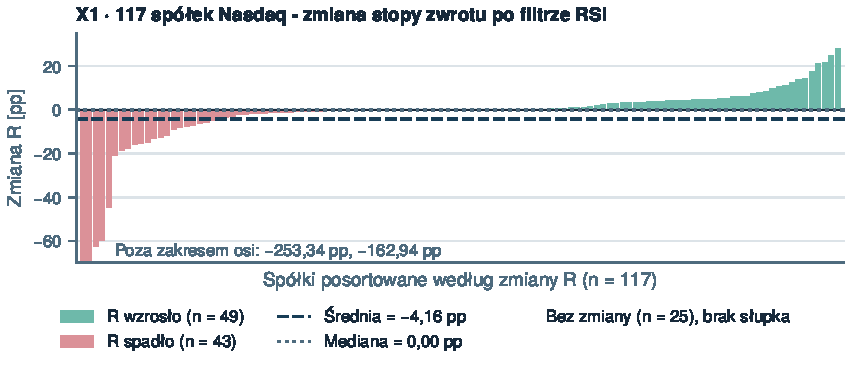
\includegraphics{X1.pdf}\par
  \vskip1mm
  Pomógł w \resExpHelpedCount{}, zaszkodził w \resExpHurtCount{}, a
  w \resExpSameCount{} nic nie zablokował.
\end{frame}

\begin{frame}
  \frametitle{Filtr usunął \resExpBlockedCount{} transakcji, ale prawie nie zmienił
    największych strat}
  \renewcommand{\arraystretch}{1.25}
  \begin{tabular*}{\textwidth}{@{}l@{\extracolsep{\fill}}rr@{}}
    \toprule
    Wielkość (wszystkie \resExpCount{} spółek) & Algorytm podstawowy
      & Z filtrem RSI \\
    \midrule
    Średnia stopa zwrotu R [\%] & \resExpMeanBasicPct & \resExpMeanModifiedPct \\
    Liczba zamkniętych transakcji & \resExpBasicClosedCount
      & \resExpModifiedClosedCount \\
    Skuteczność [\%] & \resExpBasicWinRatePct & \resExpModifiedWinRatePct \\
    Średnia największa strata [\%] & \resExpBasicMeanMaxLossPct
      & \resExpModifiedMeanMaxLossPct \\
    \midrule
    Kup i trzymaj, średnia stopa zwrotu [\%]
      & \multicolumn{2}{c@{}}{\resExpMeanHoldPct} \\
    \bottomrule
  \end{tabular*}
  \vskip3mm
  Filtr nie zmienia stopy zwrotu pozostawionych transakcji, tylko usuwa
  wejścia. Wartości dotyczą całego zbioru, nie pojedynczego przypadku.
\end{frame}

\begin{frame}[b]
  \frametitle{Zablokowane wejścia nie były gorsze od przeciętnych}
  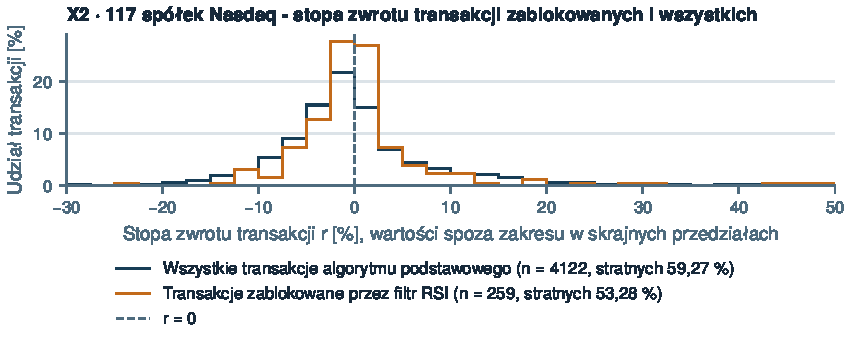
\includegraphics{X2.pdf}\par
  \vskip1mm
  Stratnych było \resExpBlockedLosingSharePct{}\,\% transakcji zablokowanych
  wobec \resExpBasicLosingSharePct{}\,\% wszystkich. Średnia stopa zwrotu
  transakcji to \resExpBlockedMeanPct{}\,\% wobec \resExpAllTradesMeanPct{}\,\%.
\end{frame}

\begin{frame}
  \frametitle{Przykłady lokalne wybrano tak, by zmiana wyniku spółki wynikała
    z jednej transakcji}
  \begin{itemize}
    \item Kryterium: spółki z dokładnie jedną zablokowaną transakcją, czyli
      \resExpSingleBlockedCount{} z \resExpCount{}. To inna grupa niż spółki
      bez zmian z wykresu X1.
    \item Filtr nie zmienia stopy zwrotu pozostawionych transakcji, więc
      zmiana R takiej spółki wynika tylko z pominiętej transakcji. Kod
      sprawdza to dla wszystkich spółek, liczba niezgodności to
      \resExpIdentityFailureCount{}.
    \item Przykład poprawy to największa dodatnia zmiana R w tej grupie,
      przykład pogorszenia to największa ujemna.
    \item Każdy przykład to jedna spółka, więc nie przesądza o wyniku całego
      zbioru.
  \end{itemize}
\end{frame}

\begin{frame}[b]
  \frametitle{\resExpHelpTicker: po kupnie przy RSI \resExpHelpRsi{} cena spadła,
    więc filtr pomógł}
  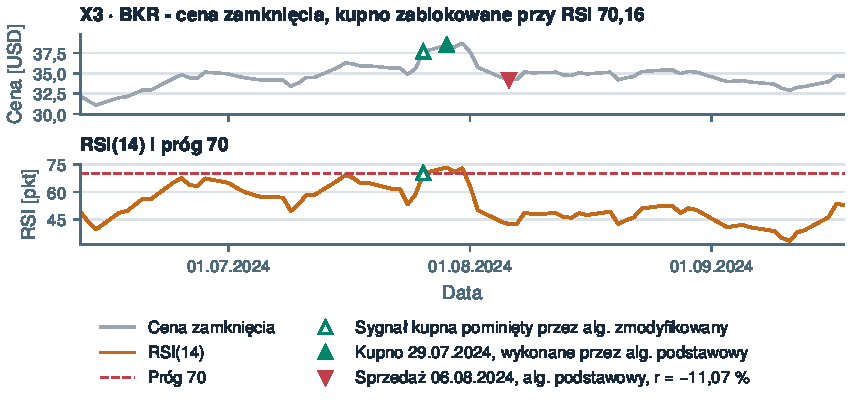
\includegraphics{X3.pdf}\par
  Bez transakcji z r = \resExpHelpReturnPct{}\,\% R spółki wzrosło
  z \resExpHelpBasicPct{}\,\% do \resExpHelpModifiedPct{}\,\%.
\end{frame}

\begin{frame}[b]
  \frametitle{\resExpHurtTicker: mimo RSI \resExpHurtRsi{} wzrost trwał dalej,
    więc filtr zaszkodził}
  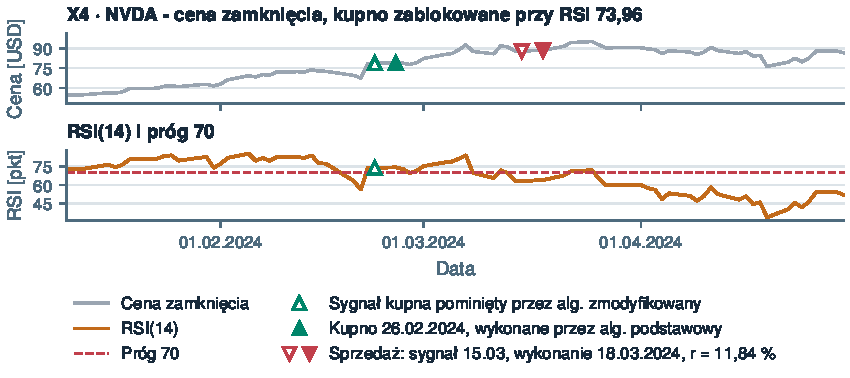
\includegraphics{X4.pdf}\par
  Bez transakcji z r = \resExpHurtReturnPct{}\,\% R spółki spadło
  z \resExpHurtBasicPct{}\,\% do \resExpHurtModifiedPct{}\,\%.
\end{frame}

\begin{frame}
  \frametitle{Próg RSI \resExpRsiThreshold{} nie odróżniał złych wejść MACD
    od dobrych}
  \begin{itemize}
    \item Obserwacja: filtr pomógł w \resExpHelpedCount{} spółkach, zaszkodził
      w \resExpHurtCount{}, a zablokowane transakcje wypadły nieco lepiej niż
      przeciętne (\resExpBlockedMeanPct{}\,\% wobec \resExpAllTradesMeanPct{}\,\%).
    \item Wyjaśnienie (hipoteza): RSI od \resExpRsiThreshold{} przy sygnale
      kupna MACD oznacza silny impet, który na rosnącym rynku często trwa
      dalej.
    \item Wniosek: filtr nie dał systematycznej poprawy, a średnią zmianę R
      (\resExpMeanDeltaPp{} pp) zaniżyło kilka dużych spadków.
    \item Zakres: \resExpCount{} spółek z dostarczonego zbioru i jeden próg
      RSI(\resExpRsiPeriod{}) w kodzie. Inne warianty sprawdzono tylko wstępnie
      przy wyborze kierunku.
  \end{itemize}
\end{frame}
